\shorthandoff{"}
\chapter{Verwandte Arbeiten}
\label{ch:verwandteArbeiten}
% Todo: Überleitung zwischen Überschriften optimieren
Bei der Durchsicht der Literatur ist festzustellen, dass bereits zahlreiche Publikationen den Anspruch verfolgten, Empfehlungssysteme zur automatisierten Bestimmung des \acp{PJFit} zu entwickeln. Jedoch bezogen sich einige Forscher dabei nicht auf das in Kapitel \ref{ch:personEnvironmentFit} vorgestellte Konzept der Psychologie. Obwohl der Begriff des \acp{PJFit} verwendet wurde, bestimmten die Wissenschaftler die Kongruenz häufig ausschließlich auf der Ebene des Anforderungen-Fähigkeiten Fits. Dieser Sachverhalt ist beispielsweise in den Veröffentlichungen von \textcite[S. 1ff.]{luo:2019}, \textcite[S. 1ff.]{qin:2018} und \textcite[S. 1ff.]{personJobFit:2018} zu beobachten.

\section{Nicht auf dem PE-Fit basierende Systeme}
\label{ch:verwandteArbeiten:nichtAufDemPEFitBasierend}
\textcite[S. 1, Z. 1f.]{personJobFit:2018} definierten den \ac{PJFit} als den "Prozess, bei dem das richtige Talent mit der richtigen Stelle zusammengeführt wird, indem die Talentkompetenzen identifiziert werden, welche für die Stelle erforderlich sind."\footnote{"process of matching the right talent for the right job by identifying talent competencies that are required for the job." - \textcite[S. 1, Z. 1f.]{personJobFit:2018}} Dementsprechend implementierten \textcite[S. 1ff.]{personJobFit:2018} wie auch \textcite[S. 1ff.]{luo:2019} und \textcite[S. 1ff.]{qin:2018} ein neuronales Netz, welches voraussagte, ob eine Person aufgrund ihrer Qualifikationen für eine Stelle geeignet ist. Auf der ersten Ebene bereiteten die Wissenschaftler unstrukturierte Stellenausschreibungen und Lebensläufe strukturiert auf. Anschließend nutzen sie die Daten, um über verschiedene Verfahren vorauszusagen, ob eine ausreichende Übereinstimmung zwischen den Fähigkeiten der Kandidaten und den Anforderungen der offenen Stellen vorhanden ist \cite[S. 1ff.]{luo:2019}\cite[S. 1ff.]{qin:2018}\cite[S. 1ff.]{personJobFit:2018}.

Empfehlungssysteme, welche neben den Präferenzen der Personalsachbearbeiter an die Fähigkeiten potentieller Mitarbeiter auch die Vorlieben der Kandidaten berücksichtigen, bezeichneten \textcite[S. 4]{malinowski:2006} als bilaterale Empfehlungssysteme. Solche Anwendungen beziehen folglich neben dem Anforderungen-Fähigkeiten Fit auch die Bedürfnisse-Angebote Kongruenz in den Vorschlagsprozess ein. Im Umfeld von \textcite[S. 1ff.]{malinowski:2006} entwickelten verschiedene Forschergruppen zwei bilaterale Recommender Engines, welche in mehreren Publikationen vorgestellt wurden. In beiden Fällen bezogen sich die Wissenschaftler auf das in Kapitel \ref{ch:personEnvironmentFit} vorgestellte Konzept des \acp{PEFit} \cite[S. 4f.]{keim:2007}\cite[S. 3f.]{keim:2005}\cite[S. 3f.]{malinowski:2005}\cite[S. 3f.]{malinowski:2006}\cite[S. 3ff.]{malinowski:2008}.

\section{Auf dem PE-Fit basierende bilaterale Systeme}
\label{ch:verwandteArbeiten:aufDemPEFitBasierendeBilateraleSysteme}
Eine der beiden bilateralen Anwendungen aus dem Umfeld von \textcite[S. 1ff.]{malinowski:2006} verfolgte das Ziel, neue Personen für bestehende Teams zu empfehlen. Zu diesem Zweck sagten die Wissenschaftler voraus, wie sehr sich potentielle Teammitglieder gegenseitig vertrauen würden. Dabei schlugen sie diejenigen Kandidaten für das Team vor, bei welcher der höchste gegenseitige Vertrauenswert zwischen bestehenden Teamkollegen und potentiellem Mitglied berechnet wurde \cite[S. 5ff.]{keim:2005}\cite[S. 1ff.]{malinowski:2005}. Das zweite System sollte Empfehlungen zur Besetzung offener Stellen generieren und dabei Präferenzen von Arbeitssuchenden und Personalsachbearbeitern beachten \cite[S. 1ff.]{malinowski:2006}. Darüber hinaus stellte \textcite[S. 5ff.]{keim:2007} ein Framework vor, welches auf beide Ansätze innerhalb einer Anwendung integrierte. Alle diese Implementierungsmethoden basieren auf einem von \textcite[S. 6ff.]{faerber:2003} vorgestellten Empfehlungssystem.

\subsection{Empfehlungssystem für Personalsachbearbeiter}
\label{ch:verwandteArbeiten:aufDemPEFitBasierendeBilateraleSysteme:grundlegendesEmpfelungssystem}
\textcite[S. 4ff.]{faerber:2003} entwickelten eine Recommender Engine zur Empfehlung von Personen für offene Stellen in Unternehmen. Dabei verfolgten sie einen hybriden, nicht-bilateralen Ansatz. Dieser ist in Abbildung \ref{fig:verwandteArbeiten:abb1} modelliert.

\begin{figure}[h]
	\centering
	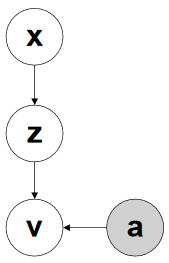
\includegraphics[width=0.3\textwidth]{gfx/faerber.png}
	\caption{Modell des hybriden Empfehlungssystems von \textcite[S. 8]{faerber:2003}}
	\label{fig:verwandteArbeiten:abb1}
\end{figure}

In Abbildung \ref{fig:verwandteArbeiten:abb1} steht $a$ für die Attribute des Bewerbers, welche beispielsweise aus dessen Lebenslauf gewonnen wurden. Variable $x$ symbolisiert einen Personalsachbearbeiter mitsamt eines Stellenprofils, welches dieser besetzen soll. Dessen Entscheidung, ob ein Bewerber für die Tätigkeit qualifiziert ist oder nicht, wurde über den boolschen Wert $v$ ausgedrückt. \textcite[S. 4ff.]{faerber:2003} bestimmten aus diesen Faktoren ein latentes Variablenmodell. Hierbei wurden bekannte Entscheidungen eines Personalsachbearbeiters hinsichtlich der Eignung von Bewerbern für eine Stelle erfasst. Aus diesen wurden nicht direkt messbare Variablen $z$ abgeleitet, welche dessen Beurteilungen beeinflussten. Über die latenten Variablen $z$ und die Attribute $a$ bestimmten die Wissenschaftler Wahrscheinlichkeiten, mit welchen ein Personalsachbearbeiter die vorliegenden Attribute eines Kandidaten als qualifiziert oder unqualifiziert bewerten würde \cite[S. 4ff.]{faerber:2003}.

Diesen Empfehlungsansatz nutzten \textcite[S. 4f.]{malinowski:2006} als Grundlage für ein neues Empfehlungssystem. Die Wissenschaftler stellten in ihrer Publikation eine bilaterale Anwendung vor, welche neben den Präferenzen der Personalsachbearbeiter auch die Vorlieben der Kandidaten berücksichtigen sollte.

\subsection{Einbeziehung der Präferenzen der Kandidaten}
\label{ch:verwandteArbeiten:aufDemPEFitBasierendeBilateraleSysteme:einbeziehungKandidaten}
Um neben den Präferenzen der Personalsachbearbeiter auch die Vorlieben der Kandidaten zu berücksichtigen, erweiterten \textcite[S. 4f.]{malinowski:2006} das von \textcite[S. 4ff.]{faerber:2003} entwickelte Empfehlungssystem um eine zusätzliche Komponente für Stellensuchende. Diese orientierte sich ebenfalls am Aufbau von Abbildung \ref{fig:verwandteArbeiten:abb1}. Bei der neuen Komponenten stand $x$ für den Kandidaten und $a$ für die Attribute der Stellenausschreibung. Auch hier bestimmten die Forscher latente Variablen $z$, welche sie über vergangene Stellenprofil-Bewertungen von Studenten ermittelten. Über diese sagten sie voraus, mit welcher Wahrscheinlichkeit ein Kandidat eine Stelle als passend zu seinen Präferenzen bewerten würde \cite[S. 4f.]{malinowski:2006}.

Bei einer Evaluation des Systems stellten \textcite[S. 6f.]{malinowski:2006} fest, dass die Ergebnisse der Komponente zur Empfehlung von Kandidaten nahezu vergleichbar zur manuellen Auswahl eines menschlichen Personalsachbearbeiters waren. Auch beim Stellenempfehlungssystem kamen die Wissenschaftler zu der Erkenntnis, dass die Ergebnisse bis auf einzelne Ausnahmen vergleichbar zur manuellen Selektion der Kandidaten waren. \textcite[S. 7]{keim:2007} bestätigte in seiner Publikation ebenfalls, dass beide Empfehlungsmodule eine hohe Genauigkeit aufweisen konnten.

Die Art der Evaluation von \textcite[S. 6f.]{malinowski:2006} muss kritisch betrachtet werden. Die Wissenschaftler prüften, ob die Ergebnisse ihrer Anwendung vergleichbar mit den Entscheidungen von Menschen waren. Hierbei hinterfragten sie jedoch nicht, ob die Auswahl der Nutzer optimal war und es somit grundsätzlich erstrebenswert war, diese Entscheidungen maschinell nachzubilden. Außerdem validierten die Forscher nicht, ob die Ergebnisse bilateraler Empfehlungssysteme tatsächlich qualitativ besser waren als die Resultate unilateraler Vorgehen. Somit bleibt ungewiss, ob der höhere Implementierungsaufwand für bilaterale Systeme in er Praxis lohnenswert ist.

Darüber hinaus ist zum Vorgehen von \textcite[S. 3ff.]{malinowski:2006} festzustellen, dass das bilaterale Empfehlungssystem ursprünglich in Anlehnung an das Konzept des \acp{PEFit} entwickelt wurde. Dabei sollten sowohl Präferenzen von Personalsachbearbeitern als auch Vorlieben von Stellensuchenden berücksichtigt werden. Allerdings ist es in der vorgestellten Anwendung nur möglich, entweder zu den Präferenzen von Personalsachbearbeitern passende Kandidaten oder mit den Vorlieben von Bewerbern kompatible Stellen zu ermitteln. Es ist nicht vorgesehen, Kandidaten für Positionen zu empfehlen und dabei gleichzeitig die Präferenzen von Bewerbern und Personalsachbearbeitern zu berücksichtigen. Daher ist kritisch anzumerken, dass die Anwendung von \textcite[S. 3ff.]{malinowski:2006} zwar die Präferenzen beider Parteien berücksichtigte, dieses Vorgehen aber nicht vollständig der Theorie des \acp{PEFit} entspricht.

Ein Empfehlungssystem, welches eher das Konzept des \acp{PEFit} erfüllte, stellten \textcite[S. 1ff.]{malinowski:2005} in einer anderen Publikation vor.

\subsection{System zur bilateralen Vertrauensbestimmung}
\label{ch:verwandteArbeiten:aufDemPEFitBasierendeBilateraleSysteme:bilateraleVertrauensbestimmung}
\textcite[S. 1]{malinowski:2005} präsentierten eine Recommender Engine, welche Personen für Teams vorschlagen sollte. Einerseits berücksichtigten die Wissenschaftler hierbei die Präferenzen von Personalsachbearbeitern hinsichtlich der fachlichen Eignung der Kandidaten. Andererseits beachteten sie auch die Präferenzen von Teammitgliedern und potentiellen Kandidaten bezüglich der persönlichen Zusammenarbeit.

Um dieses Ziel zu erreichen, sah es das System von \textcite[S. 4ff.]{malinowski:2005} in einem ersten Schritt vor, das Verfahren von \textcite[S. 8ff.]{faerber:2003} aus Kapitel \ref{ch:verwandteArbeiten:aufDemPEFitBasierendeBilateraleSysteme:grundlegendesEmpfelungssystem} anzuwenden. Über dieses bestimmten die Wissenschaftler aus allen verfügbaren Kandidaten die $N$ fachlich geeignetsten Personen passend zu den Präferenzen des Personalsachbearbeiters. Diese dienten als Eingabe für eine weitere Komponente, über welche die Wissenschaftler das gegenseitige Vertrauen zwischen den $N$ Kandidaten und den vorhanden Teammitgliedern berechneten. Um dieses zu bestimmen, nutzten die Forscher drei separate Ansätze. Diese sind in Abbildung \ref{fig:verwandteArbeiten:abb2} dargestellt und wurden auch in den Publikationen von \textcite[S. 5ff.]{keim:2005} und \textcite[S. 6ff.]{malinowski:2008} behandelt.

\begin{figure}[h]
	\centering
	
	\subfloat[Transitive Beziehung]{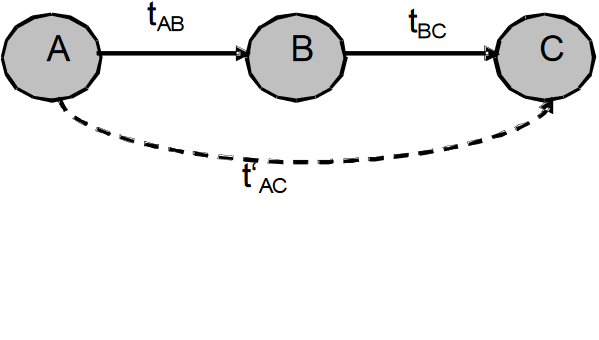
\includegraphics[width = 0.33\textwidth]{gfx/trustmodelA.png}}
	\subfloat[Kollaboratives Filtern]{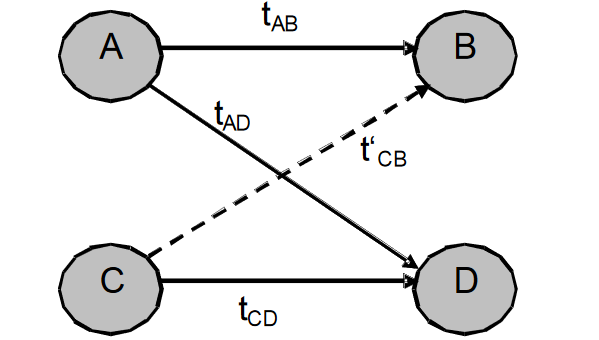
\includegraphics[width = 0.33\textwidth]{gfx/trustmodelB.png}}
	\subfloat[Ähnlichkeitsberechnung über latente Variablen]{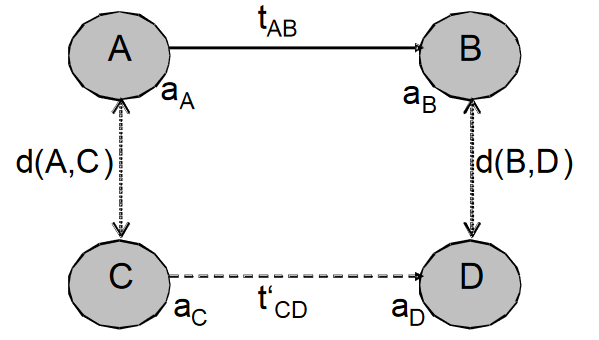
\includegraphics[width = 0.33\textwidth]{gfx/trustmodelC.png}}
	
	\caption{Ansätze zur Berechnung des Vertrauens zwischen potentiellen Teammitgliedern \cite[S. 5]{malinowski:2005}}
	\label{fig:verwandteArbeiten:abb2}
\end{figure}

Die Anwendung der ersten beiden Ansätze (a) und (b) zur Vorhersage des Vertrauens zwischen potentiellen Teammitgliedern aus Abbildung \ref{fig:verwandteArbeiten:abb2} setzt laut \textcite[S. 4ff.]{malinowski:2005} voraus, dass bekannte Vertrauensbewertungen von Teamkollegen vorhanden sind. Diese können den Wissenschaftlern zu Folge beispielsweise über Fragebögen ermittelt werden.

Bei Ansatz (a) nahmen \textcite[S. 5f.]{malinowski:2005} an, dass eine Vertrauensbeziehung über Multiplikation berechnet werden kann, wenn transitiv eine direkte Verbindung zwischen zwei Personen besteht. Zur Berechnung der Vertrauensbeziehung $t'_{AC}$ von Person A zu Person C in Abbildung \ref{fig:verwandteArbeiten:abb2} wendeten die Wissenschaftler folgende Formel \ref{frml:verwandteArbeiten:formel1} an:
\begin{equation}
	t'_{AC} = t_{AB} * t_{BC}
	\label{frml:verwandteArbeiten:formel1}
\end{equation}
Ansatz (b) in Abbildung \ref{fig:verwandteArbeiten:abb2} zeigt die Berechnung des Vertrauens zwischen zwei Personen über speicherbasiertes kollaboratives Filtern, wie es in Kapitel \ref{ch:empfehlungssysteme:cf} vorgestellt wurde. Hierbei nutzten die Wissenschaftler die Ähnlichkeit zwischen den Personen A und C, um den Vertrauenswert zwischen den Personen C und B vorherzusagen \cite[S. 6]{malinowski:2005}.

Das dritte Verfahren (c) beruhte auf der Annahme, dass sich Personen stark vertrauen würden, wenn sie ähnliche persönliche Präferenzen teilen. Unter dieser Prämisse erstellten \textcite[S. 6f.]{malinowski:2005} ein latentes Variablenmodell vergleichbar zum Verfahren aus Kapitel \ref{ch:verwandteArbeiten:aufDemPEFitBasierendeBilateraleSysteme:einbeziehungKandidaten}. Über dieses bestimmten sie für jedes Teammitglied diejenigen latenten Variablen, welche für dieses bei der Bewertung vergangener Stellen besonders wichtig waren. Die ermittelten latenten Variablen und die gemeinsam bewerteten Stellenprofile nutzten die Wissenschaftler, um über die Ähnlichkeit zwischen Personen auf deren gegenseitiges Vertrauen zu schließen.

Die aus den drei Ansätzen (a), (b) und (c) erhaltenen Vertrauenswerte zwischen bestehenden Teammitgliedern und potentiellen Kandidaten aggregierten \textcite[S. 7ff.]{malinowski:2005} unter Berücksichtigung der Anzahl gemeinsam bewerteter Stellenprofile zu einer finalen Vertrauensbewertung.

Im letzten Schritt des Systems errechneten \textcite[S. 9f.]{malinowski:2005} aus den Ergebnissen der Komponente von \textcite[S. 8ff.]{faerber:2003} und der finalen Vertrauensbewertung eine gemeinsame Ergebnisliste. Hierzu wendeten sie die folgende Formel \ref{frml:verwandteArbeiten:formel2} an:
\begin{equation}
	R' = \alpha * t'_{M*y} * (1-\alpha) * r'_{x,y,v}
	\label{frml:verwandteArbeiten:formel2}
\end{equation}
In Formel \ref{frml:verwandteArbeiten:formel2} stand $t'_{M*y}$ für die Liste der Vertrauensbeziehungen und $r'_{x,y,v}$ für die fachlichen Bewertungen der Kandidaten. Für $\alpha$ setzten die Wissenschaftler den Wert 0.5 ein \cite[S. 4ff.]{malinowski:2005}. Kritisch merkten \textcite[S. 9]{malinowski:2005} zu Formel \ref{frml:verwandteArbeiten:formel2} an, dass diese noch nicht optimal sei und weiterer Forschung bedarf.

Eine Evaluation des Gesamtsystems konnte in der Literatur nicht identifiziert werden. In der Publikation von \textcite[S. 13ff.]{malinowski:2008} findet sich lediglich eine Validierung der Komponente zur Berechnung des Vertrauens zwischen Teammitgliedern und potentiellen Kandidaten. Hierbei kamen die Wissenschaftler zu der Erkenntnis, dass deren System eine höhere Genauigkeit als ein zufälliges Vorhersagesystem aufweisen konnte. Allerdings merkten die Forscher zu ihrer Testgruppe an, dass diese mit 21 Teilnehmern zu klein sei, um signifikante Resultate zu erzielen.

Die Berechnung der gegenseitigen Vertrauensbeziehungen zwischen bestehenden Teammitgliedern und potentiellen Kandidaten nutzte auch \textcite[S. 1ff.]{keim:2007}. Er präsentierte ein Framework, welches Personen in passende Projektteams einordnen und dabei sowohl Fähigkeiten als auch zwischenmenschliche Attribute berücksichtigen sollte.

\subsection{Framework zur Bestimmung von Person-Job und Person-Team Fit}
\label{ch:verwandteArbeiten:aufDemPEFitBasierendeBilateraleSysteme:pjUndPtFit}
Das von \textcite[S. 1ff.]{keim:2007} vorgestellte Framework ist in Abbildung \ref{fig:verwandteArbeiten:abb3} dargestellt. Es bestand aus drei Ebenen.

\begin{figure}[h]
	\centering
	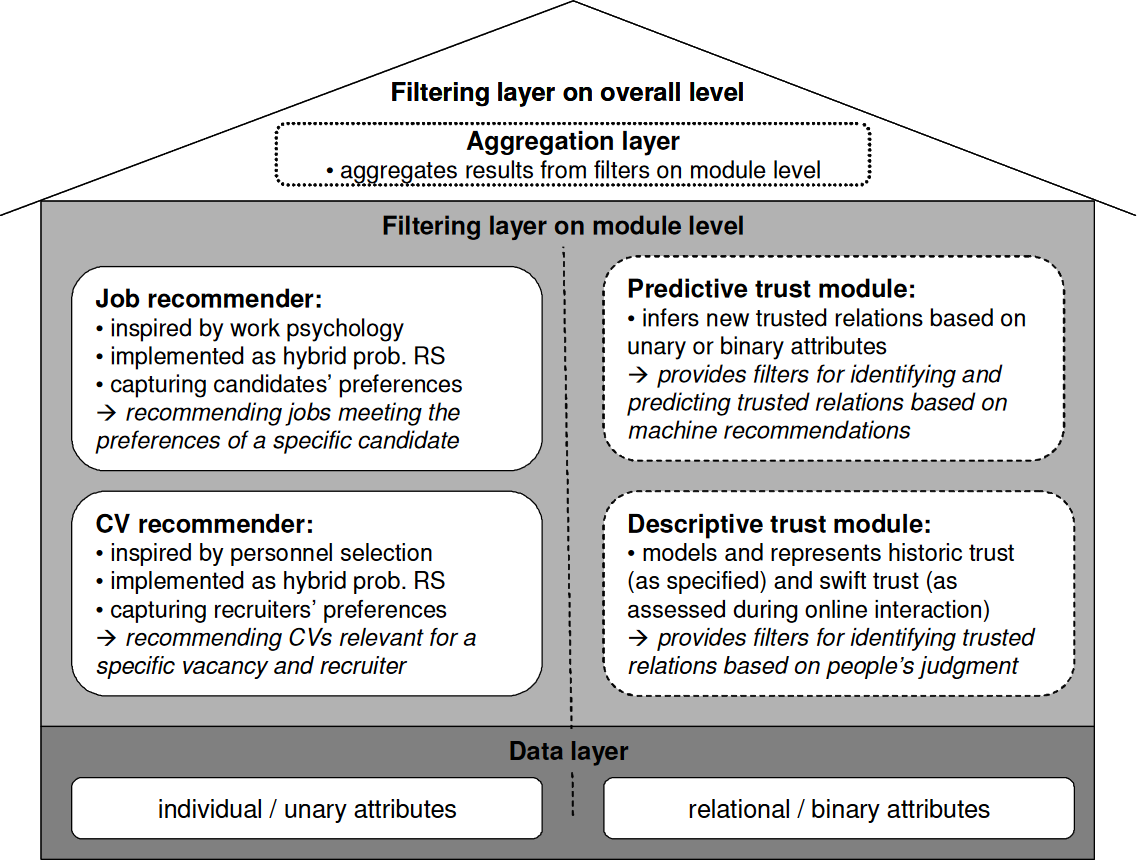
\includegraphics[width=0.85\textwidth]{gfx/keim-multilayer.png}
	\caption{Framework von \textcite[S. 5]{keim:2007}}
	\label{fig:verwandteArbeiten:abb3}
\end{figure}

% Diese entsprachen den in den vorherigen Kapiteln behandelten Anwendungen von \textcite[S. 6ff.]{faerber:2003}, \textcite[S. 4ff.]{keim:2005}, \textcite[S. 4ff.]{malinowski:2005} und \textcite[S. 3ff.]{malinowski:2006}. 
In Abbildung \ref{fig:verwandteArbeiten:abb3} ist zu erkennen, dass die zweite Ebene des Frameworks von \textcite[S. 5ff.]{keim:2007} aus vier Komponenten bestand. Diese sollten die Daten, welche auf der ersten Ebene gespeichert waren, laden und entsprechend ihrer Funktion filtern. Dabei sollten die beiden auf der linken Seite abgebildeten Module die Stellen- bzw. Kandidatensuche unterstützen. Die Komponenten der rechten Seite sollten die Bestimmung geeigneter Teampartner erleichtern \cite[S. 5]{keim:2007}.

Das Lebenslaufempfehlungssystem (CV recommender) in Abbildung \ref{fig:verwandteArbeiten:abb3} entsprach der von \textcite[S. 8ff.]{faerber:2003} entwickelten Anwendung, welche in Kapitel \ref{ch:verwandteArbeiten:aufDemPEFitBasierendeBilateraleSysteme:grundlegendesEmpfelungssystem} vorgestellt wurde \cite[S. 6]{keim:2007}. Beim Stellenempfehlungssystem (Job recommender) handelte es sich um die von \textcite[S. 4ff.]{malinowski:2006} adaptierte Version des Lebenslaufempfehlungssystems, mit welcher Personen zu ihren Präferenzen passende Stellenausschreibungen ermitteln konnten \cite[S. 6]{keim:2007}. Dieses wurde in Kapitel \ref{ch:verwandteArbeiten:aufDemPEFitBasierendeBilateraleSysteme:einbeziehungKandidaten} behandelt. Das vorhersagende Vertrauensmodul (Predictive Trust module) entsprach dem in Kapitel \ref{ch:verwandteArbeiten:aufDemPEFitBasierendeBilateraleSysteme:bilateraleVertrauensbestimmung} behandelten Ansatz zur Vorhersage von Vertrauensbeziehungen zwischen potentiellen Teammitgliedern \cite[S. 8]{keim:2007}. Dieses wurde in den Publikationen von \textcite[S. 5ff.]{keim:2005} und \textcite[S. 4ff.]{malinowski:2005} detailliert vorgestellt.

Vergleichbar zu einer Anwendung von \textcite[S. 4f.]{keim:2005} ist auch das beschreibende Vertrauensmodul (Descriptive trust module). Diese Komponente erfasste explizit vergebene Vertrauensbewertungen von Teammitgliedern in Form einer Ontologie und repräsentierte diese in Form eines Graphen. Über diese Darstellung konnten Anwender soziale Beziehungen durchsuchen und analysieren. Auf diese Weise sollten sie besser entscheiden können, mit welchen Personen sie eine Zusammenarbeit eingehen möchten \cite[S. 7]{keim:2007}.

Ähnlich zur Publikation von \textcite[S. 3ff.]{malinowski:2006} muss auch zur Veröffentlichung von \textcite[S. 5ff.]{keim:2007} kritisch bemerkt werden, dass die Forscher die Resultate der einzelnen Module nicht zu einem Ergebnis zusammenfassten. Die Implementierung der oben in Abbildung \ref{fig:verwandteArbeiten:abb3} dargestellten Aggregationsebene (Aggregation layer) ließen die Wissenschaftler in ihrer Publikation offen \cite[S. 8]{keim:2007}.
%Das von \textcite{keim:2007} vorgestellte System enthielt mit dem beschreibenden und dem vorhersagenden Vertrauensmodul somit zwar Komponenten, welche bilaterale Vertrauensbeziehungen modellieren bzw. bei der Empfehlungsbestimmung berücksichtigten. Damit handelte es sich bei der Suche nach potentiell vertrauenswürdigen Teamkollegen um einen bilateralen Prozess, da Präferenzen von bestehenden Teammitgliedern und potentiellen Kandidaten berücksichtigt wurden. Es wurde jedoch nicht beachtet, ob die Person auch fachlich für die Stelle geeignet war oder ob die Position inhaltlich den Vorstellungen des Kandidaten entsprach.

Neben denen in diesem Kapitel vorgestellten Publikationen wurden bei der Literaturrecherche weitere Ansätze identifiziert, bilaterale Empfehlungssysteme zu implementieren. Die Autoren dieser Veröffentlichungen bezeichneten ihre Anwendungen jedoch nicht als bilateral sondern als wechselseitig. % Quellen
%Zusammenfassend ist zu den Publikationen aus dem Umfeld von \textcite[S. 1ff.]{malinowski:2006} festzustellen, dass diese einige Empfehlungssysteme mit Bezug auf den \ac{PEFit} entwickelten. Deren Anwendungen unterstützten insbesondere die Auswahl fachlich geeigneter Stellen bzw. Kandidaten und die Zusammenführung einzelner Personen mit bestehenden Teams. Jedoch muss kritisch bemerkt werden, dass die einzelnen Module meist keine bilateralen Empfehlungen generierten. Eine dafür benötigte Integration der einzelnen Ansätze wurde nur in Ausnahmefällen wie beispielsweise von \textcite[S. 4ff.]{malinowski:2005} vorgenommen. Diese wählten Kandidaten entsprechend der fachlichen Präferenzen von Personalsachbearbeitern aus und sortieren diese unter Beachtung des gegenseitigen Vertrauens mit den potentiellen Teammitgliedern. In den vorliegenden Publikationen konnte keine Methode identifiziert werden, bei welcher eine Anwendung Stellen passend zu den fachlichen Präferenzen von Personalsachbearbeitern und Kandidaten bestimmte.

\section{Wechselseitige Empfehlungssysteme zum Person-Job Fit}
\label{ch:verwandteArbeiten:nichtAufDemPEFitBasierendeBilateraleSysteme}
Der Begriff der wechselseitigen Empfehlungssysteme wurde erstmals von \textcite[S. 1]{pizzato:2010} eingeführt, welche eine Recommender Engine im Bereich des Online-Datings entwickelten \cite[S. 1]{wenxing:2015}. Die Autoren verwendeten dabei die Bezeichnung der Wechselseitigkeit, da ihr System sowohl die Präferenzen des aktiven Nutzers als auch der potentiellen Partner gleichermaßen berücksichtigen sollte \cite[S. 1]{pizzato:2010}. In ihrer Publikation nannten \textcite[S. 3]{pizzato:2010} die Veröffentlichung von \textcite[S. 1ff.]{malinowski:2006} als verwandte Arbeit. Hierzu stellten sie fest, dass auch bilaterale Empfehlungssysteme die Präferenzen von zwei Parteien betrachten. Eine klare Unterscheidung zwischen bilateralen und wechselseitigen Empfehlungssystemen nahmen die Autoren jedoch nicht vor \cite[S. 3]{pizzato:2010}. Erst in einer späteren Publikation hielten \textcite[S. 8]{pizzato:2013} eindeutig fest, dass wechselseitig und bilateral zwei unterschiedliche Begriffe für dasselbe Konzept von Empfehlungssystemen sind.

Wechselseitige Empfehlungssysteme zum \ac{PJFit} wurden unter anderem von \textcite[S. 1ff.]{ding:2016}, \textcite[S. 1ff.]{wenxing:2015} und \textcite[S. 1ff.]{lu:2013} vorgestellt. Diese Autoren bezogen sich nicht auf das Konzept des \acp{PEFit}. Dennoch entwickelten sie Systeme, welche sowohl Präferenzen von Stellensuchenden als auch Personalsachbearbeitern gleichermaßen in den Vorschlagsprozess einbezogen. 

\subsection{System zur Einstellung von Hochschulabsolventen}
\label{ch:verwandteArbeiten:nichtAufDemPEFitBasierendeBilateraleSysteme:absolventen}
\textcite[S. 1ff.]{ding:2016} entwickelten ein wechselseitiges Empfehlungssystem zur Einstellung von Hochschulabsolventen. Zur Empfehlung geeigneter Stellen für Kandidaten griff das System auf Informationen über den Nutzer und ehemalige Absolventen der Universität zu. Stellenempfehlungen wurden hierbei über ein mehrstufiges Verfahren bestimmt. Dieses berechnete die Ähnlichkeit des Kandidaten zu vergangenen Absolventen und nutzte deren Stellenentscheidungen als Grundlage für Vorschläge.

Zur Empfehlung geeigneter Absolventen für Arbeitgeber lud die Anwendung Informationen über ehemalige Graduierende der Universität, welche nach dem Studium in diesem Unternehmen eine Tätigkeit begonnen hatten. Auch in diesem Fall wurde das mehrstufige Verfahren angewendet, welches als Grundlage für die Empfehlungen die Ähnlichkeit der historischen Absolventen zu den Daten aktueller Graduierender verwendete \cite[S. 1ff.]{ding:2016}.
% Hierbei griffen sie auf historische Daten einer Universität zurück. Die Anwendung erlaubte es Absolventen Profile mit Stellenpräferenzen und Arbeitgebern Profile mit Stellenanforderungen zu erstellen. 

Kritisch ist zum Vorgehen von \textcite[S. 1ff.]{ding:2016} anzumerken, dass die Autoren aus der Anstellung eines Absolventen unmittelbar auf gegenseitige Präferenzen von Arbeitgebern und Graduierenden schlossen. Jedoch könnte ein Berufseinsteiger auch eine weniger präferierte Stelle angenommen haben, da dessen Wunschposition nicht verfügbar war oder mit einem anderen Kandidaten besetzt wurde. Ebenso könnte ein Arbeitgeber einen weniger passenden Absolventen eingestellt haben, da kein idealer Bewerber vorhanden war oder sich dieser für einen anderen Arbeitgeber entschieden hatte.

Positiv ist zu zum Vorgehen von \textcite[S. 1ff.]{ding:2016} anzumerken, dass deren Anwendung mit sehr vielen impliziten Daten arbeitete. Somit war es für Anwender beispielsweise nicht notwendig, umfangreiche Fragebögen vor der initialen Verwendung des Systems auszufüllen.

\subsection{Wechselseitige Empfehlungen mittels Kosinus-Distanz}
\label{ch:verwandteArbeiten:nichtAufDemPEFitBasierendeBilateraleSysteme:nutzer}
Ein weiteres wechselseitiges Empfehlungssystem zur Stellenbesetzung stellten \textcite[S. 1ff.]{wenxing:2015} vor. Dieses System richtete sich an Personalsachbearbeiter und Stellensuchende. Wie in Abbildung \ref{fig:verwandteArbeiten:nichtAufDemPEFitBasierendeBilateraleSysteme:abb1} dargestellt, teilte die Anwendung die hinterlegten Informationen der beiden Gruppen von Nutzern in die Kategorien Selbstbeschreibung (Self-description) und Präferenz (Preference).

\begin{figure}[h]
	\centering
	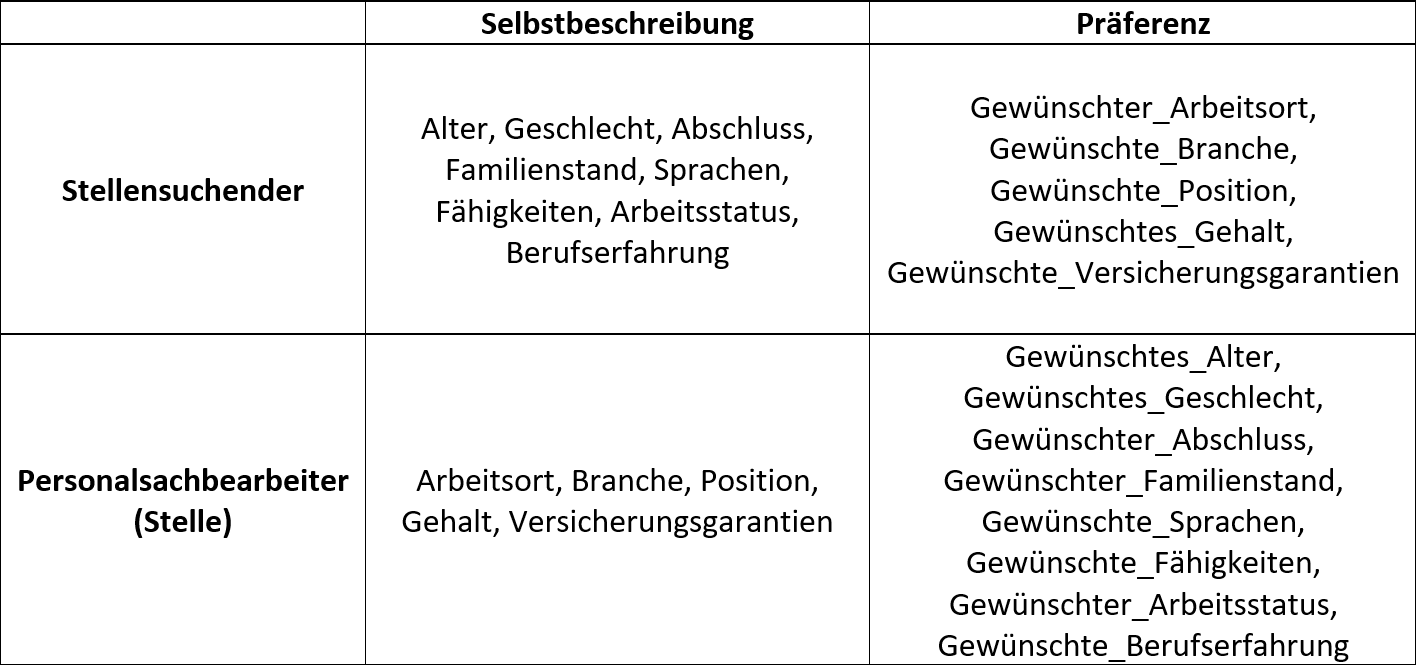
\includegraphics[width=0.7\textwidth]{gfx/hong-tabelle.png}
	\caption{Tabelle mit Merkmalskategorien im wechselseitigen Empfehlungssystem von \textcite[S. 2]{wenxing:2015}}
	\label{fig:verwandteArbeiten:nichtAufDemPEFitBasierendeBilateraleSysteme:abb1}
\end{figure}

Wie in Abbildung \ref{fig:verwandteArbeiten:nichtAufDemPEFitBasierendeBilateraleSysteme:abb1} zu erkennen, entsprach jedes Merkmal in der Selbstbeschreibung der Jobsuchenden einem Merkmal der Präferenzen der Personalsachbearbeiter und umgekehrt. Vorschläge berechnete das Empfehlungssystem über die Kosinus-Ähnlichkeit, welche anhand von Gleichung \ref{fig:empfehlungssysteme:cf:speicherbasiert:formel1} in Kapitel \ref{ch:empfehlungssysteme:cf:speicherbasiert} vorgestellt wurde. Zur Berechnung der Gleichartigkeit stellte die Anwendung die Merkmale der Nutzer in Form von Vektoren dar. Zur Vorschlagsbestimmung für Stellensuchende bestimmte das System im ersten Schritt die Ähnlichkeit zwischen der Selbstbeschreibung des zugreifenden Anwenders und den Präferenzen aller verfügbaren Personalsachbearbeiter. In einem zweiten Schritt wurde die Ähnlichkeit zwischen den Selbstbeschreibungen aller Personalsachbearbeiter und den Präferenzen des zugreifenden Nutzers bestimmt. In einem letzten Schritt addierte das System die in den beiden vorherigen Rechenschritten erhaltenen Ähnlichkeiten zwischen zugreifendem Nutzer und Personalsachbearbeitern auf. Anschließend gab es die $N$ HR-Mitarbeiter zurück, bei welchen die höchste Gleichartigkeit mit dem Stellensuchenden bestimmt werden konnte. Die Berechnung der relevantesten Kandidaten aus Sicht der Personalsachbearbeiter wurde analog durchgeführt \cite[S. 2f.]{wenxing:2015}.

Positiv ist zum Vorgehen von \textcite[S. 1ff.]{wenxing:2015} anzumerken, dass dieses das Konzept des \acp{PEFit} sehr exakt erfüllte, auch wenn sich die Wissenschaftler nicht direkt auf diese Theorie bezogen. So fand auf Seiten beider Anwendergruppen eine eindeutige Einteilung in Nachfrage- und Angebotsperspektive statt, welche bei der Berechnung von Empfehlungen gleichermaßen berücksichtigt wurden.

Kritisch ist festzustellen, dass die in Abbildung \ref{fig:verwandteArbeiten:nichtAufDemPEFitBasierendeBilateraleSysteme:abb1} dargestellten Präferenzen von den Nutzern nicht, wie in Kapitel \ref{ch:personEnvironmentFit:wichtigkeiten} behandelt, gewichtet wurden. Somit arbeitete das Empfehlungssystem mit der impliziten Prämisse, dass jede ermittelte Präferenz gleich wichtig sei. Außerdem wurde nicht evaluiert, ob das wechselseitige Empfehlungssystem wie geplant zu einer "win-win Situation"\footnote{"win-win situation" - \textcite[S. 3, Z. 45f.]{wenxing:2015}} \cite[S. 3, Z. 45f.]{wenxing:2015} führte. So wäre es auch denkbar, dass das System statt eines gemeinsamen optimalen Ergebnisses einen kleinsten gemeinsamen Nenner bestimmte, mit welchem weder Stellensuchende noch Personalsachbearbeiter zufrieden wären.

Eine Evaluation führten lediglich \textcite[S. 1ff.]{hong:2013b} mit einem Vorgängersystem der vorgestellten Anwendung durch. Hierbei bestimmten die Wissenschaftler wechselseitige Empfehlungen mit einem hybriden System, welches die Ergebnisse von kollaborativem Filtern, inhaltsbasiertem Filtern und einem Greedy-Algorithmus kombinierte. In der Evaluation verglichen die Wissenschaftler die Nutzererfahrung ihres wechselseitigen Empfehlungssystems dem rein klassischen kollaborativen und rein inhaltsbasierten Filtern anhand einer Nutzerstudie. Das wechselseitige Empfehlungssystem wurde hierbei in den Punkten Interpretierbarkeit, Diversität und Sortierung besser als die beiden anderen Methoden bewertet. Unter dem Gesichtspunkt der Relevanz stuften die Nutzer die Ergebnisse des wechselseitigen Empfehlungssystems jedoch lediglich als ähnlich relevant zu den Resultaten des klassischen kollaborativen Filterns ein. Somit ist fraglich, ob die Realisierung des wechselseitigen Empfehlungssystems aus wirtschaftlicher Sicht lohnenswert war.

Außerdem muss kritisiert werden, dass die Bewertungen nicht nach Nutzergruppen aufgeschlüsselt wurden. Somit ist nicht feststellbar, ob die Ergebnisse von Personalsachbearbeitern und Stellensuchenden voneinander abwichen.

Im Sinne des \acp{PEFit} muss darüber hinaus angemerkt werden, dass die Relevanz für sämtliche Nutzer anhand gleicher Fragen erhoben wurde. Somit kann nicht festgestellt werden, ob das wechselseitige Empfehlungssystem die Erkenntnisse der Psychologen aus Kapitel \ref{ch:personEnvironmentFit:supplementaryUndComplementary} bestätigen konnte. Deren Forschungen zu Folge führt ein \ac{PEFit} aus Sicht der Personalsachbearbeiter zu einer guten Arbeitsleistung und aus Perspektive der Angestellten zu einer hohen Zufriedenheit.

\section{Graphenbasiertes Empfehlungssystem}
\label{ch:verwandteArbeiten:nichtAufDemPEFitBasierendeBilateraleSysteme:lu:2013}
% Dieses System berücksichtigt Präferenzen von Kandidaten und Arbeitgebern
% Hybrid, da Profilähnlichkeit (Contentbased) und Kollaboratives Filtern
Ein weiteres Empfehlungssystem präsentierten \textcite[S. 1ff.]{lu:2013}. Die Wissenschaftler generierten Vorschläge über einen graphenbasierten Ansatz unter Beachtung der Interessen von Kandidaten und Arbeitgebern. Ihr System bezeichneten sie jedoch weder explizit als wechselseitig, noch als bilateral. \textcite[S. 1ff.]{lu:2013} erstellten ein Jobportal auf Basis eines Graphen, in welchem Stellensuchende, Arbeitgeber und Jobausschreibungen, wie Abbildung \ref{fig:verwandteArbeiten:nichtAufDemPEFitBasierendeBilateraleSysteme:lu:2013:abb1} dargestellt, in Form von Knoten existierten.

\begin{figure}[h]
	\centering
	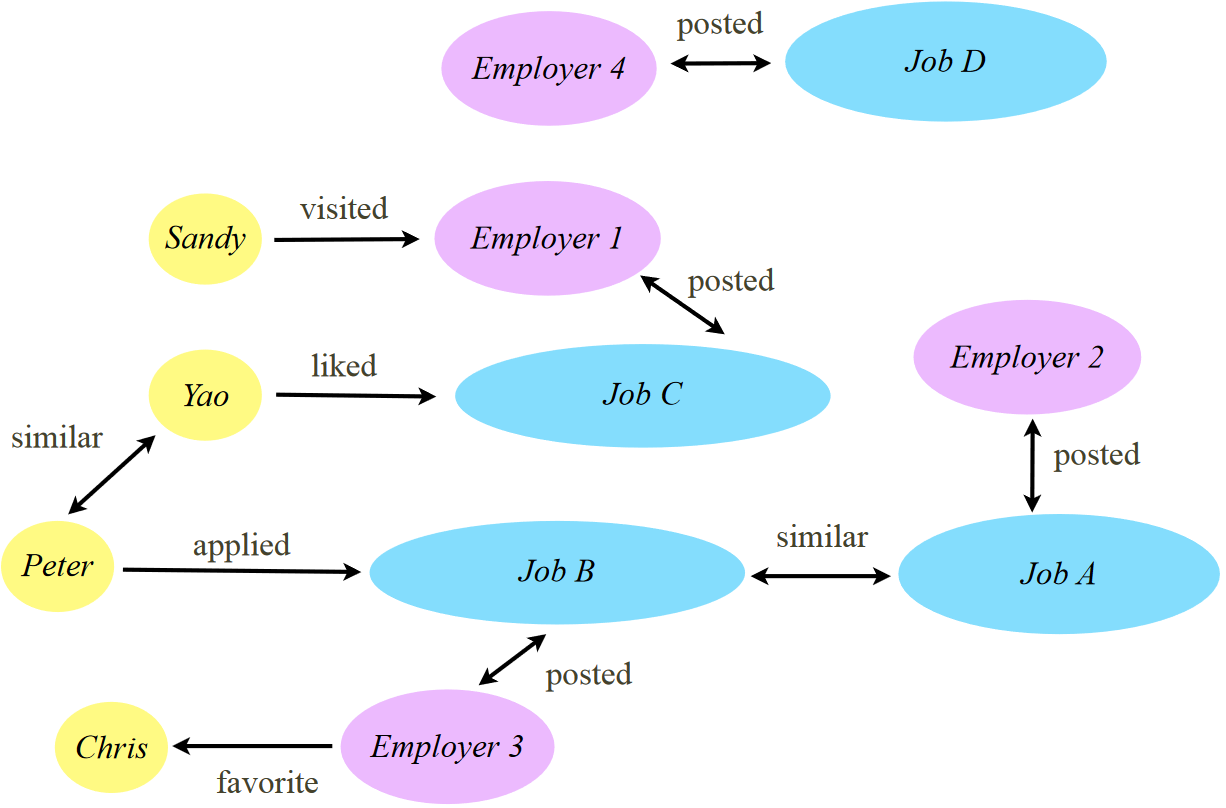
\includegraphics[width=0.9\textwidth]{gfx/lu-graph.png}
	\caption{Graphenstruktur des wechselseitigen Empfehlungssystems von \textcite[S. 2]{lu:2013}}
	\label{fig:verwandteArbeiten:nichtAufDemPEFitBasierendeBilateraleSysteme:lu:2013:abb1}
\end{figure}

Kanten wurden im Graphen aus Abbildung \ref{fig:verwandteArbeiten:nichtAufDemPEFitBasierendeBilateraleSysteme:lu:2013:abb1} für jede Interaktionen zwischen den Entitäten, wie dem Besuch eines Profils oder dem Bewerben auf eine Stelle, angelegt. Zusätzlich verfügte jede der dargestellten Entitäten über textuelle Profilbeschreibungen. Diese nutzten die Wissenschaftler als Grundlage für inhaltsbasierte Verfahren. Über diese bestimmten sie die Gleichartigkeit von Profilen und fügten bei hoher Ähnlichkeit zusätzliche Kanten hinzu. Dieses Vorgehen half den Wissenschaftlern die Problematik des Kaltstars zu beheben. Jede Kante erhielt ein bestimmtes Gewicht, sodass beispielsweise das Bewerben auf eine Stelle höher gewertet wurde als der Besuch eines Profils \cite[S. 1ff.]{lu:2013}.

Ein auf dem PageRank basierender Algorithmus unterstützte Stellensuchende und Arbeitgeber auf Grundlage des Graphen bei der Auswahl geeigneter Ausschreibungen bzw. Kandidaten. In die Berechnung wurde ein Personalisierungsfaktor einbezogen, welcher die Wichtigkeit der direkten Nachbarn eines Zielknotens erhöhte. In der finalen Ergebnisliste entfernte das System die direkten Nachbarn, um dem Nutzer ausschließlich Elemente zu empfehlen, welche diesem bislang unbekannt waren \cite[S. 3]{lu:2013}.

In einer Evaluation verglichen \textcite[S. 3f.]{lu:2013} die Genauigkeit ihres hybriden Systems mit den Ergebnissen des reinen kollaborativen und inhaltsbasierten Filterns. Hierbei stellten sie fest, dass ihr hybrider Empfehlungsansatz meist präzisere Ergebnisse liefern konnte als die beiden anderen Verfahren. Jedoch ist insbesondere bei der Empfehlung von Kandidaten für offene Stellen eine hohe Streuung in den Ergebnissen zu beobachten. So erzielte das hybride Empfehlungssystem bei dem Vorschlagen von Kandidaten für ein Stellenprofil eine Genauigkeit von 70 Prozent, während die inhaltsbasierte Recommender Engine lediglich 30 Prozent erzielte. Bei einem anderen Stellenprofil erreichte der hybride Ansatz dagegen nur eine Genauigkeit von 20 Prozent, während das inhaltsbasierte Verfahren 80 Prozent erzielte. Auf Ursachen für diese Abweichungen gingen die Wissenschaftler in ihrer Publikation nicht ein.

Kritisch muss zur Evaluation außerdem festgestellt werden, dass die Genauigkeit der Empfehlungen den Forschern zu Folge manuell verifiziert wurden. Wie dieser Prozess ablief wird in der Veröffentlichung nicht erläutert. Somit ist es nicht eindeutig feststellbar, ob das Empfehlungssystem wie beim \ac{PEFit} prognostiziert, auf Seiten der Kandidaten zu einer ausgeprägteren Zufriedenheit und aus Sicht der Unternehmen zu einer höheren Leistung führte.

Positiv ist zum Vorgehen von \textcite[S. 1ff.]{lu:2013} zu bemerken, dass diese mit sehr vielen impliziten Bewertungen arbeiteten. So ist der zu erwartende manuelle Nutzeraufwand zur Pflege von Präferenzen sehr gering.

Abschließend kann hinterfragt werden, ob die impliziten Daten zu aussagekräftigeren Ergebnissen führen als explizit hinterlegte Informationen. So wäre es vorstellbar, dass ein Nutzer häufig die Profile von Stellen oder Arbeitgebern besucht, bei welchen dieser nicht explizit ausdrücken kann, weshalb er diese präferiert. Hier könnte ein latentes Variablenmodell helfen, solche impliziten Vorlieben explizit festzustellen und in den weiteren Empfehlungsprozess einzubeziehen.
\shorthandon{"}
